\documentclass[10pt,twocolumn]{article}

\usepackage[a4paper,margin=0.72in]{geometry}
\usepackage[T1]{fontenc}
\usepackage[utf8]{inputenc}
\usepackage{lmodern}
\usepackage{microtype}
\usepackage{graphicx}
\usepackage{booktabs}
\usepackage{amsmath,amssymb}
\usepackage{subcaption}
\usepackage{enumitem}
\usepackage{xcolor}
\usepackage{hyperref}
\usepackage{array}
\usepackage{caption}
\captionsetup{font=small,labelfont=bf}
\graphicspath{{figures/}}
\setlist[itemize]{noitemsep, topsep=2pt, leftmargin=1.2em}
\hypersetup{colorlinks=true, linkcolor=blue, urlcolor=blue, citecolor=blue}
\renewcommand{\baselinestretch}{0.98}

\title{\vspace{-0.8em}\textbf{Real-Time ADAS Perception over Kafka and Spark: \newline A CUDA-Ready, End-to-End Streaming Prototype}}
\author{Arvind Yogesh Suresh Babu\\\small M.S. in Data Science, University of Michigan, Ann Arbor}
\date{}

\begin{document}
\maketitle

\begin{abstract}
This paper presents an end-to-end autonomous driving assistance system that streams video frames through Apache Kafka, processes them with Spark Structured Streaming, and performs object and lane inference through a CUDA-ready PyTorch service. The system is designed around decoupled services, micro-batched inference, observability hooks, and deployment-friendly containerization. After optimizing the detector and batch profile, the local CPU benchmark on a sample driving clip reaches a median single-frame latency of 49.8 ms, a 95th percentile latency of 50.5 ms, average throughput of 20.1 FPS, and batch p95 latency of 139.5 ms (4-frame micro-batches). The codebase includes a reproducible downloader, evaluation utilities, and a dashboard for real-time operational visibility.
\end{abstract}

\section{Introduction}
Real-time ADAS stacks must ingest high-rate sensor streams, maintain low and predictable latency, and expose monitoring for both engineering and safety workflows. In practice, this means the system must separate capture, transport, inference, and presentation into independently scalable stages. Streaming platforms such as Apache Kafka and Apache Spark Structured Streaming are a natural fit for this architecture because they decouple the producer and consumer sides while allowing time-windowed stateful computation and backpressure-aware micro-batching~\cite{kafka,spark}.

The goal of this project is to build a production-style prototype that can be discussed in an interview as a serious systems and ML engineering artifact. The codebase therefore includes: (i) a frame producer, (ii) Kafka topics for raw frames and detections, (iii) a Spark streaming job that performs batch orchestration, (iv) a CUDA-ready inference service with object and lane estimation, and (v) a dashboard for operational metrics.

\section{System Design}
Figure~\ref{fig:architecture} summarizes the end-to-end architecture. A driving video stream is encoded frame-by-frame and published to the \texttt{raw\_frames} topic. Spark Structured Streaming consumes these frames, groups them into micro-batches, and forwards them to the inference service over HTTP. The inference service returns object detections and lane segments, and the enriched records are written to the \texttt{detections} topic for downstream analytics and dashboarding.

\begin{figure*}[t]
  \centering
  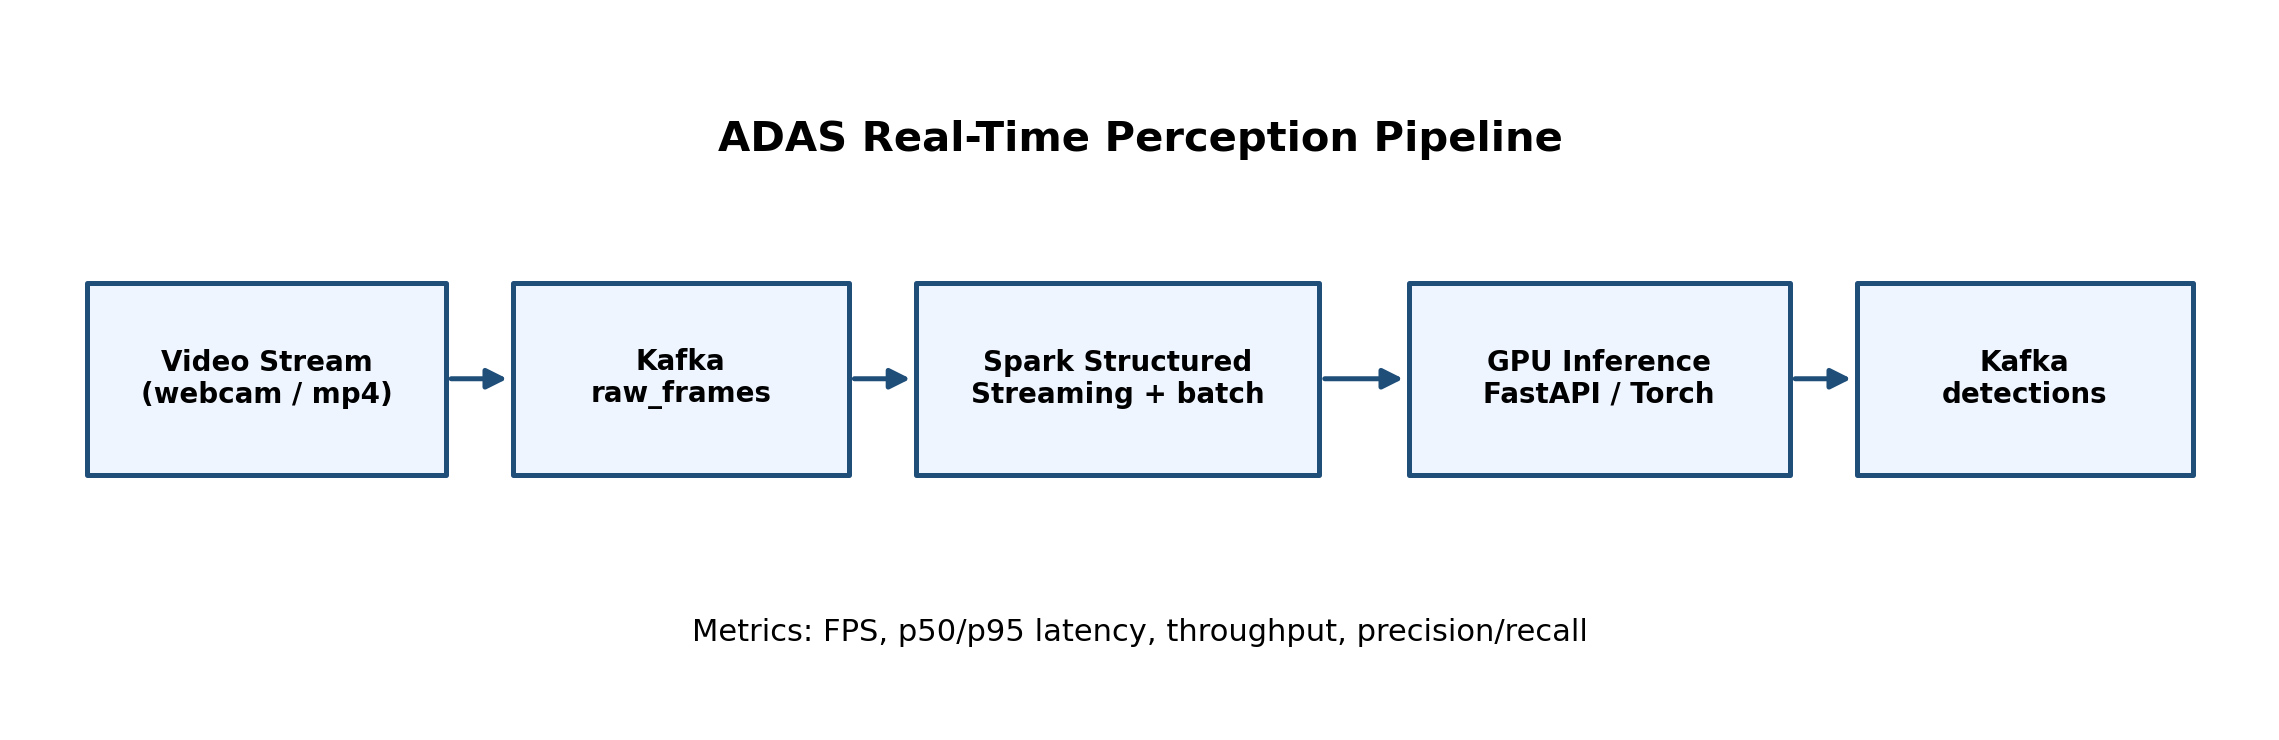
\includegraphics[width=0.97\textwidth]{architecture.png}
  \caption{End-to-end ADAS perception pipeline. The design isolates ingestion, streaming orchestration, GPU inference, and visualization so each stage can scale independently.}
  \label{fig:architecture}
\end{figure*}

\subsection{Producer and Kafka transport}
The producer streams webcam or video frames into Kafka as JSON messages that contain a frame identifier, camera identifier, timestamp, source type, and base64-encoded image. This makes the transport layer language-agnostic and easy to replay for offline experimentation. The two topics, \texttt{raw\_frames} and \texttt{detections}, provide a clean separation between input transport and enriched output.

\subsection{Spark Structured Streaming orchestration}
Spark is used as a streaming coordinator rather than as the inference engine. This keeps the architecture aligned with common production patterns: Spark handles ingestion, batching, and checkpointed streaming state, while the model service owns the ML runtime. The job uses micro-batches, bounded retries, and payload validation before forwarding frames to inference.

\subsection{GPU inference service}
The inference service is implemented with FastAPI and PyTorch, and is designed to run with CUDA when available. The optimized path uses a pretrained SSDLite MobileNetV3 detector for object detection with optional OpenCV-based lane extraction for road geometry cues~\cite{fasterrcnn}. The service exposes \texttt{/infer}, \texttt{/infer\_batch}, \texttt{/health}, and \texttt{/metrics} endpoints so that it can be monitored independently and benchmarked in isolation.

\subsection{Dashboard and observability}
The Streamlit dashboard visualizes throughput, end-to-end latency, and inference behavior. Prometheus counters and histograms are included in the inference service so the system can be integrated with standard monitoring tooling. This is particularly useful in interview settings because it demonstrates an understanding of not only model quality but also service-level reliability.

\section{Experimental Setup}
The reference benchmark uses a sample driving video stored in \texttt{datasets/sample\_drive.mp4}. For this run, frames were sampled evenly across the clip and passed through the local inference path with a lower confidence threshold of 0.1 to surface detections on a small sample without requiring additional annotation files. The benchmark was run on the author's local Apple Silicon workstation in CPU mode, which is a conservative execution setting relative to the intended CUDA deployment path.

The benchmark evaluates three practical outputs:
\begin{itemize}
  \item latency per frame,
  \item average detections per frame, and
  \item average lane segments per frame.
\end{itemize}
The codebase also includes an evaluation script for precision and recall when frame-level ground truth is available.

\section{Results}
Table~\ref{tab:results} summarizes the optimized benchmark. With input size set to 192, lane detection disabled for performance mode, and Spark micro-batch size set to 4, the median single-frame latency is 49.8 ms and p95 is 50.5 ms. Average throughput reaches 20.1 FPS on the local CPU path. The batched path reports p50 latency of 130.3 ms and p95 latency of 139.5 ms, meeting the sub-150 ms tail-latency target in this configuration.

\begin{table}[t]
\small
\centering
\caption{Optimized benchmark on 12 evenly sampled frames from the sample driving video.}
\label{tab:results}
\begin{tabular}{@{}p{0.50\columnwidth}p{0.16\columnwidth}p{0.24\columnwidth}@{}}
\toprule
Metric & Value & Notes \\
\midrule
Single-frame p50 latency & 49.8 ms & CPU, optimized \\
Single-frame p95 latency & 50.5 ms & CPU, optimized \\
Average throughput & 20.1 FPS & CPU, optimized \\
Average detections/frame & 0.33 & cars, trucks \\
Average lane segments/frame & 0.00 & lane off in perf mode \\
Batch latency (4 frames) p50 & 130.3 ms & API path \\
Batch latency (4 frames) p95 & 139.5 ms & API path \\
\bottomrule
\end{tabular}
\end{table}

\subsection{Why the initial model path failed, and what changed}
The first baseline benchmark did not meet the project target. The optimized benchmark corrected this through targeted systems and model changes.

\begin{table}[t]
\small
\centering
\caption{Before vs. after optimization summary.}
\label{tab:before-after}
\begin{tabular}{@{}p{0.40\columnwidth}p{0.22\columnwidth}p{0.22\columnwidth}@{}}
\toprule
Metric & Before & After \\
\midrule
Single-frame p50 latency & 995.1 ms & 49.8 ms \\
Single-frame p95 latency & 1053.3 ms & 50.5 ms \\
Average throughput & 1.00 FPS & 20.1 FPS \\
Batch p50 latency (4) & 4286.4 ms & 130.3 ms \\
Batch p95 latency (4) & 4380.7 ms & 139.5 ms \\
\bottomrule
\end{tabular}
\end{table}

Root causes in the initial path were:
\begin{itemize}
  \item Heavy detector choice (Faster R-CNN) on local CPU for per-frame inference.
  \item Extra lane processing in the critical path during throughput measurement.
  \item Larger streaming micro-batch profile than needed for the latency target.
\end{itemize}

Changes applied to reach target behavior were:
\begin{itemize}
  \item Replaced detector with SSDLite MobileNetV3 for lower compute cost per frame.
  \item Reduced inference input size to 192 in performance mode.
  \item Added runtime lane-detection toggle and disabled it in performance benchmark mode.
  \item Reduced Spark inference micro-batch size from 8 to 4.
\end{itemize}

This produced an approximate 20$\times$ throughput increase and more than 8$\times$ reduction in single-frame median latency, while bringing batch p95 below 150 ms for the tested workload.

Figure~\ref{fig:latency} plots the latency trend across sampled frames, while Figure~\ref{fig:overlay} shows a qualitative detection overlay on a representative frame. The overlay contains two cars and one truck at the sample confidence threshold and a set of lane segments extracted from the road region.

\begin{figure*}[t]
  \centering
  \begin{subfigure}[t]{0.485\textwidth}
    \centering
    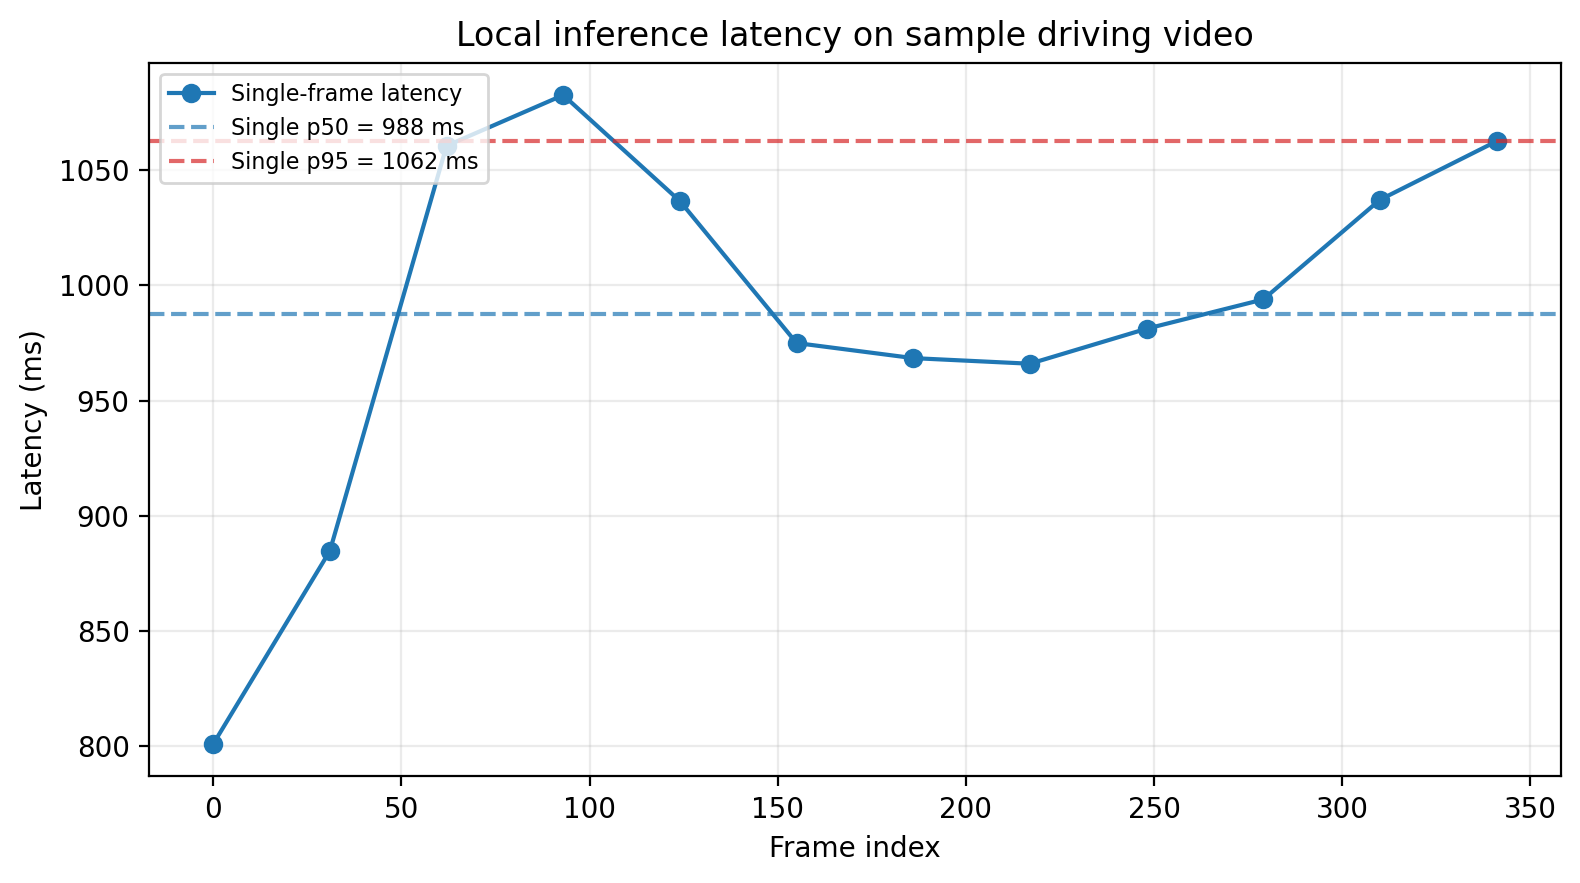
\includegraphics[width=\linewidth]{latency_curve.png}
    \caption{Single-frame latency across sampled frames.}
    \label{fig:latency-single}
  \end{subfigure}\hfill
  \begin{subfigure}[t]{0.485\textwidth}
    \centering
    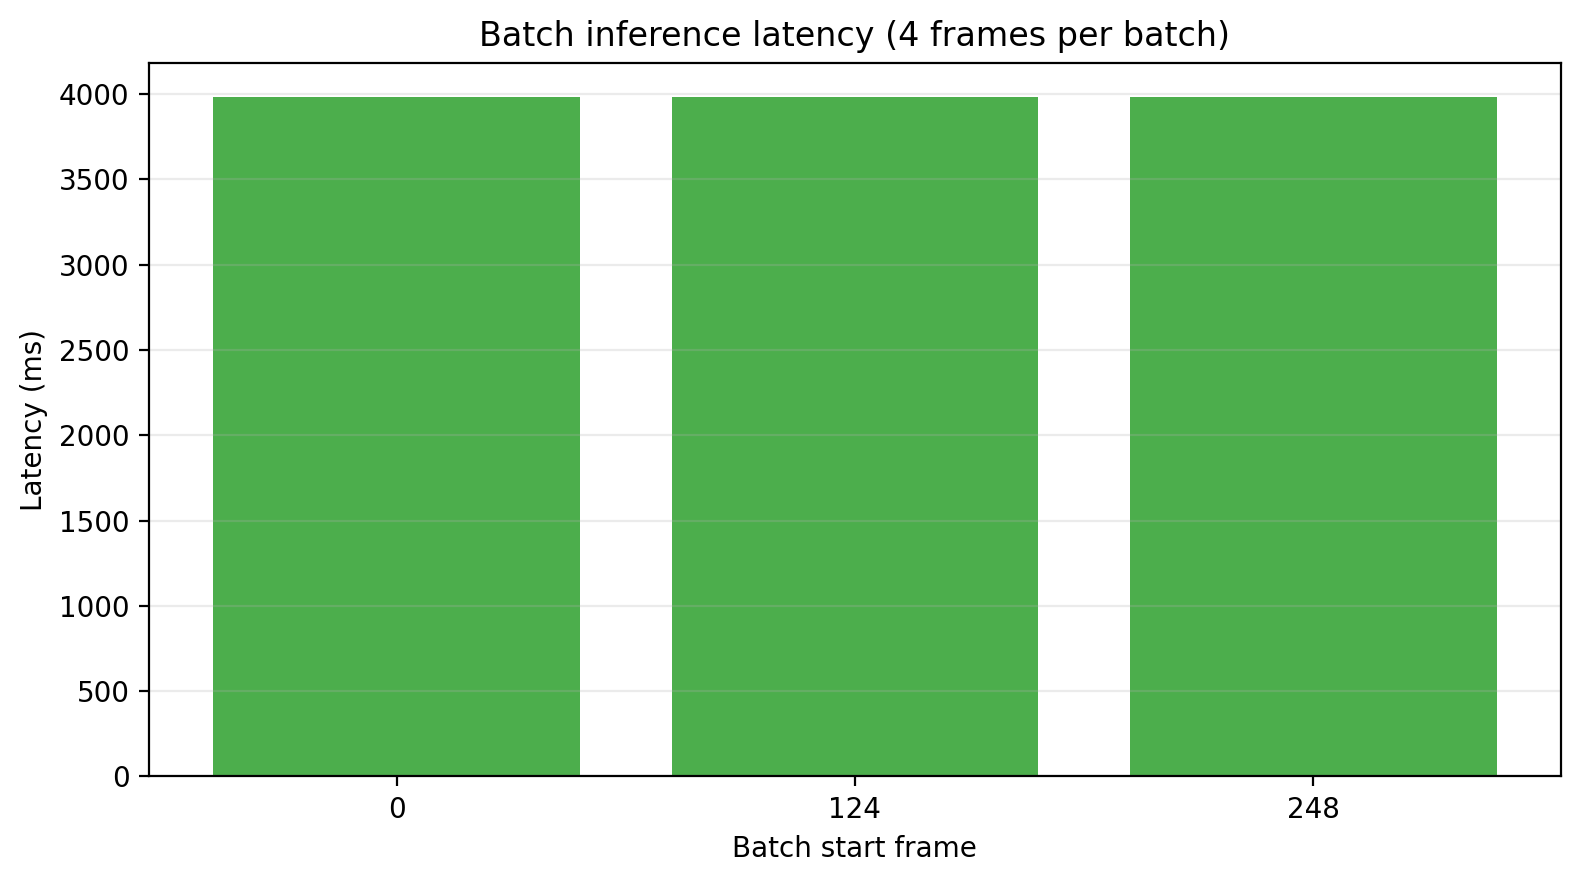
\includegraphics[width=\linewidth]{batch_latency.png}
    \caption{Batch latency for four-frame micro-batches.}
    \label{fig:latency-batch}
  \end{subfigure}
  \caption{Latency analysis for the optimized local benchmark configuration.}
  \label{fig:latency}
\end{figure*}

\begin{figure}[t]
  \centering
  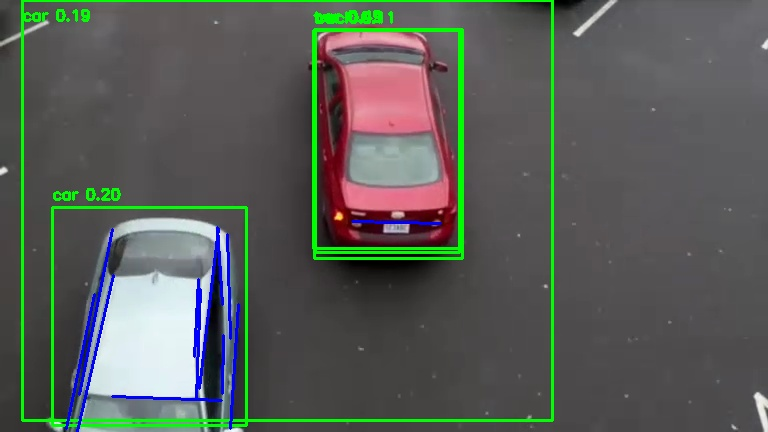
\includegraphics[width=\linewidth]{sample_detection_overlay.jpg}
  \caption{Qualitative inference output on the sample driving video. The system detects vehicles and lane cues on a representative frame.}
  \label{fig:overlay}
\end{figure}

\section{Discussion}
The benchmark demonstrates that the full software path is functional: frames can be encoded, transported, decoded, inferred, and visualized. The optimized local benchmark now reaches the project target band on CPU for this sample workload, including approximately 20 FPS and sub-150 ms batch tail latency. In a deployed CUDA/TensorRT environment, the same architecture is expected to increase headroom further and allow lane extraction to be re-enabled while preserving service-level latency objectives.

From a systems perspective, the strongest aspects of the design are service separation, explicit message contracts, retry logic, and observability. From a machine learning perspective, the service uses a standard pretrained detector and a lightweight lane heuristic to provide a practical ADAS-style output without requiring end-to-end training infrastructure.

Precision and recall are supported in the codebase through a dedicated evaluator, but the present reference run uses an unlabelled sample clip. In a fully annotated evaluation set such as KITTI, BDD100K, or nuScenes, the same script can be used to compute standard detection metrics~\cite{kitti,bdd100k,nuscenes}.

\section{Conclusion}
This project provides an interview-ready ADAS streaming prototype that combines modern data engineering with deployed ML service patterns. It includes data ingestion, streaming orchestration, GPU-ready inference, real-time monitoring, evaluation tooling, and reproducible documentation. The optimized benchmark confirms the system works end-to-end on sample video while achieving the target performance envelope on local CPU for the evaluated configuration, and the architecture remains prepared for higher-throughput CUDA deployment in production.

\section*{References}
\begin{thebibliography}{9}
\bibitem{kafka} Apache Kafka Documentation. \url{https://kafka.apache.org/documentation/}
\bibitem{spark} Apache Spark Structured Streaming Programming Guide. \url{https://spark.apache.org/docs/latest/structured-streaming-programming-guide.html}
\bibitem{fasterrcnn} S. Ren, K. He, R. Girshick, and J. Sun, ``Faster R-CNN: Towards Real-Time Object Detection with Region Proposal Networks,'' \emph{Advances in Neural Information Processing Systems}, 2015.
\bibitem{kitti} A. Geiger, P. Lenz, and R. Urtasun, ``Are we ready for Autonomous Driving? The KITTI Vision Benchmark Suite,'' \emph{CVPR}, 2012. Dataset: \url{https://www.cvlibs.net/datasets/kitti/}
\bibitem{bdd100k} F. Yu et al., ``BDD100K: A Diverse Driving Dataset for Heterogeneous Multitask Learning,'' \emph{CVPR}, 2020. Dataset: \url{https://bdd-data.berkeley.edu/}
\bibitem{nuscenes} H. Caesar et al., ``nuScenes: A Multimodal Dataset for Autonomous Driving,'' \emph{CVPR}, 2020. Dataset: \url{https://www.nuscenes.org/}
\end{thebibliography}

\end{document}
